% This LaTeX document needs to be compiled with XeLaTeX.
\documentclass[10pt]{article}
\usepackage[utf8]{inputenc}
\usepackage{amsmath}
\usepackage{amsfonts}
\usepackage{amssymb}
\usepackage[version=4]{mhchem}
\usepackage{stmaryrd}
\usepackage{graphicx}
\usepackage[export]{adjustbox}
\graphicspath{ {./images/} }
\usepackage[fallback]{xeCJK}
\usepackage{polyglossia}
\usepackage{fontspec}
\setCJKmainfont{Noto Serif CJK JP}

\setmainlanguage{polish}
\setmainfont{CMU Serif}

\title{LIGA MATEMATYCZNA im. Zdzisława Matuskiego \\
 FINAモ \\
 16 kwietnia 2018 \\
 GIMNAZJUM \\
 (klasa VII szkoły podstawowej, klasa II i III gimnazjum) }

\author{}
\date{}


\newcommand\varangle{\mathop{\sphericalangle}}

\begin{document}
\maketitle
\section*{ZADANIE 1.}
Suma 2018 liczb całkowitych jest liczbą nieparzystą. Jaką liczbą, parzystą czy nieparzystą, jest iloczyn tych liczb? Odpowiedź uzasadnij.

\section*{ZADANIE 2.}
Obecnie (w 2018 roku) ojciec i syn mają razem 131 lat. Obaj urodzili się w \(X X\) wieku. Ostatnie dwie cyfry roku urodzenia ojca stanowią liczbę będącą połową liczby utworzonej z dwóch ostatnich cyfr roku urodzenia syna. Podaj lata urodzenia ojca i syna.

\section*{ZADANIE 3.}
Wykaż, że różnica kwadratów dowolnej liczby pierwszej większej od 2 i liczby o 2 od niej mniejszej jest podzielna przez 8.

\section*{ZADANIE 4.}
Dane są dwa kwadraty o bokach \(a\) i \(b\) (jak na rysunku). Oblicz stosunek pól czworokąta \(A B C H\) i kwadratu \(A B C D\).\\
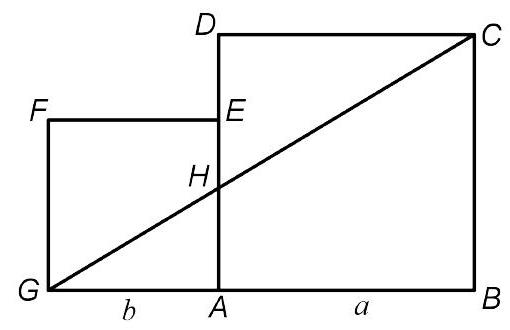
\includegraphics[max width=\textwidth, center]{2024_11_21_b25a1615f00f7e9be986g-1}

\section*{ZADANIE 5.}
Wiadomo, że punkty \(B, C\) leżą na bokach trójkąta \(A E D,|A B|=|B C|=|C D|=|D E|\) oraz \(\varangle A D E=140^{\circ}\). Wyznacz miarę kąta \(E A D\).\\
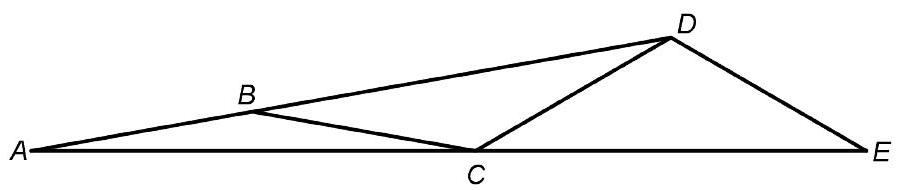
\includegraphics[max width=\textwidth, center]{2024_11_21_b25a1615f00f7e9be986g-1(1)}


\end{document}